%!TEX root = ../../Master.tex
\subsection{Google Maps}
Google Maps is a web mapping service hosted by Google inc. The application is used by some of Google's other products such as Google Transit\cite{Goo_transist}. 

\begin{figure}[ht!]
    \centering
    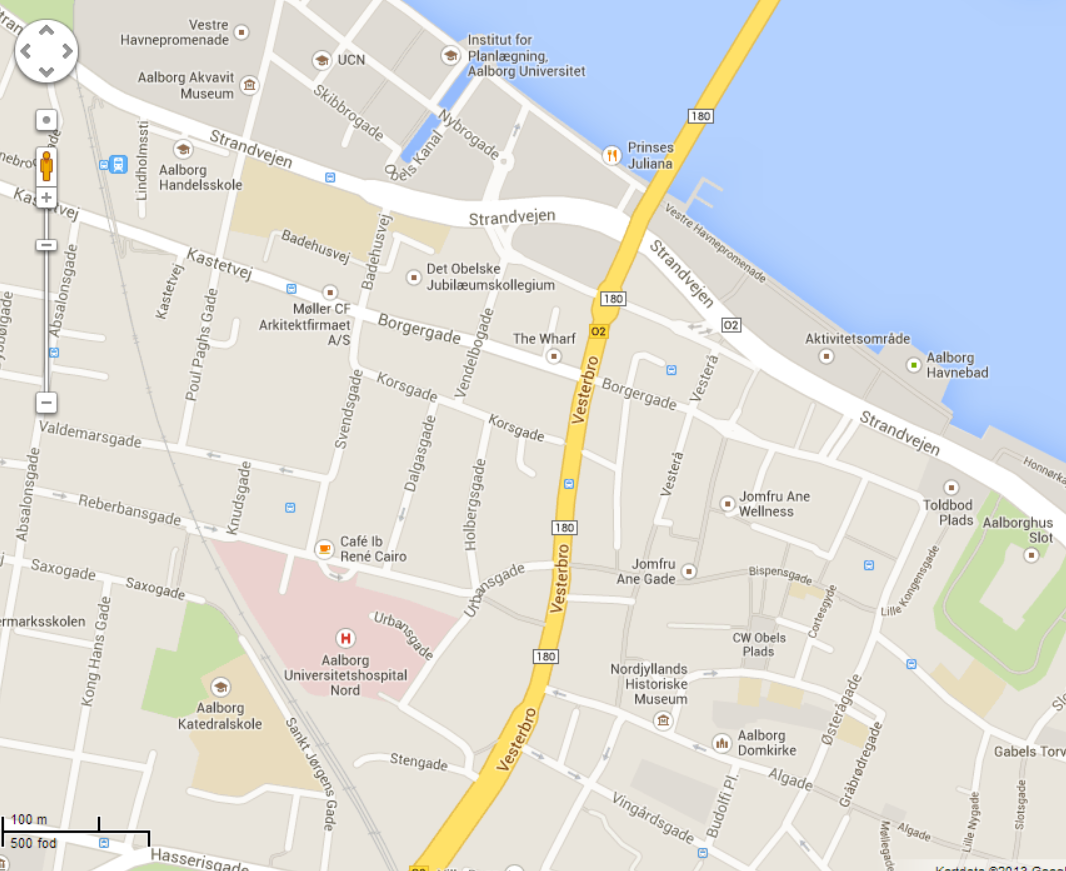
\includegraphics[width=0.6\textwidth]{google_maps}
    \caption{Google Maps}
    \label{fig:google_maps}
  \end{figure}

When a user is using on the Google maps application, all information will be downloaded to their device. Information is downloaded when they search on a location or when they drag the map around\cite{Goo_input}. The satellite images are acquired from other companies like Tele Atlas\cite{Goo_Tele} or Zenrin\cite{Goo_Zenrin} and then overlayed with Ground truth\cite{Goo_GT}.
The map will be shown with a top down view like many other maps and will offer satellite images, road maps or dynamic maps. It is also possible to go into Street View which is another Google tool, from where the viewpoint is from the street level\cite{Goo_street}.

Google maps can be used to plan routes, show earthquakes and even lets you swim with turtles\cite{Goo_Turtle}.

Google maps is relevant for this project as they have made it able to show maps inside buildings, as seen at Aalborg Universitet, Cassiopeia\cite{Goo_Indoor}. This system could be implanted at the hospital so it would show the different floors and have them all mapped. Instead of using a GPS, Google Maps Indoor uses Wi-Fi hotspots and telephone towers to locate their target\cite{Goo_Indoor}.

It is not certain that every complex has enough Wi-Fi hotspots or telephone towers nearby. Therefore this may not be a general solution.